% !TeX root = tcolorbox.tex
% include file of tcolorbox.tex (manual of the LaTeX package tcolorbox)
\clearpage
\section{Library \mylib{external}}\label{sec:external}%
\tcbset{external/prefix=external/external_}%
The library is loaded by a package option or inside the preamble by:
\begin{dispListing}
\tcbuselibrary{external}
\end{dispListing}

The purpose of this library is to support externalization of document
snippets like graphics or boxes which can be compiled stand-alone.
These snippets are written to external files, compiled and the resulting
pdf files are included to the main document as images.
The whole procedure saves compilation time, if such a snippet is costly to
compile but needs to compile just once or very seldom.

There are very good alternatives to this library. One should consider
the |standalone| package or the \tikzname\ externalization library instead.
The \mylib{external} library is something in between and can be seen as
poor man variant of the \tikzname\ externalization library.

The main differences between \tikzname\ externalization and \mylib{external} are:
\begin{itemize}
\item\tikzname\ |external| compiles the whole original document in a sophisticated
  way while \mylib{external} uses only the preamble or a part of the preamble
  of the original document.
\item\tikzname\ |external| can automatically externalize all |tikzpicture|
  environments while \mylib{external} externalizes marked snippets only.
\item Code snippets to be externalized by \mylib{external} are not restricted to
  |tikzpicture| environments. But these snippets have to be stand-alone without
  dependencies to the rest of the document.
\end{itemize}
Why should somebody use \mylib{external} instead of the more powerful \tikzname\ |external|?
One reason could be compilation speed, but the main reason for creating the
library at all was that \tikzname\ |external| tends to choke on complicated
documents where the sophisticated mechanism stumbles. Since \mylib{external} does
not use the original document body for compilation, this cannot happen.

\begin{marker}
Source snippets are compiled, if their |md5| checksum has changed.
They are not compiled automatically, if option settings are changed or
anything outside the snippet is changed.
Use \refKey{/tcb/external/force remake} to force compilation in this case
or simply delete the externalized pdf oder md5 files.
\end{marker}

\begin{marker}
To use the externalization options, the compiler has to be called with the
|-shell-escape| permission to authorize potentially dangerous system calls.
Be warned that this is a security risk.
\end{marker}


\clearpage
\subsection{Preparation of a Document for Externalization}\label{subsec:external_preparation}

The preamble of the main document has to contain the \refCom{tcbEXTERNALIZE}
command. Without this command, no externalization operation will be
executed.

\begin{docCommand}[doc new=2015-03-11]{tcbEXTERNALIZE}{}
  It is mandatory for externalization that this command is used once
  in the preamble of the main document. Every setting \emph{before}
  \refCom{tcbEXTERNALIZE} will also be used for compiling an external
  snippet. Every setting \emph{after} \refCom{tcbEXTERNALIZE} will be
  ignored for compiling an external snippet.
  Place this command right before |\begin{document}|, if you are not
  absolutely sure about another place.

  The main document has to look like the following:

\begin{dispListing}
\documentclass[a4paper]{book}%   for example
\usepackage{...}%                anything
% ...
% Tpyically, all or the very most settings for the document.

\tcbEXTERNALIZE% Typically, just before \begin{document}

% Additional settings which are ABSOLUTELY irrelevant for the
% stand-alone snippets.
%
\begin{document}
  % The document.
  % This also contains the marked snippets for externalization.
\end{document}
\end{dispListing}
\end{docCommand}

During compilation, a \refKey{/tcb/external/runner} file
is dynamically created (several times). This is the actual main file for
compiling an externalized snippet.

\begin{extTcbKey}[][doc new=2015-03-11]{runner}{=\meta{file name}}{no default,
  initially \texttt{\cs{jobname}\detokenize{_run.tex}}}
Sets the \meta{file name} for dynamically created |runner| file.
This is the actual main file for a document snippet.
Typically, the initial setting is not needed to be changed.
\begin{dispListing}
\tcbset{external/runner=myrunner.tex}
\end{dispListing}
\end{extTcbKey}

\begin{extTcbKey}[][doc new=2015-03-11]{prefix}{=\meta{text}}{no default,
  initially \texttt{external/}}
The \meta{text} is prefixed to any \refKey{/tcb/external/name} for an
externalization snippet. The initial setting implies saving all snippets
into an |external/| subdirectory. Depending on the operation system,
the subdirectory may have to be created manually once.
\begin{dispListing}
% Use a 'real' prefix instead of writing into a subdirectory:
\tcbset{external/prefix=ext_}
\end{dispListing}
\end{extTcbKey}


\begin{extTcbKey}[][doc new=2015-03-11]{externalize}{\colOpt{=true\textbar false}}{default |true|,
  initially |true|}
If set to |true|, the marked snippets are compiled if necessary.
If set to |false|, the marked snippets are not compiled but included as text.
\refKey{/tcb/external/externalize} can only be used after \refCom{tcbEXTERNALIZE}.
\end{extTcbKey}

\begin{extTcbKey}[][doc new=2015-03-11]{force remake}{\colOpt{=true\textbar false}}{default |true|,
  initially |false|}
If set to |true|, the marked snippets are always compiled.
If set to |true|, the marked snippets are compiled only if necessary.
The necessity is given, if a compiled pdf file is missing or the
|md5| checksum of the source snippet has changed.
\end{extTcbKey}

\enlargethispage*{1cm}
\begin{extTcbKey}[][doc new and updated={2015-03-11}{2017-02-24}]{\tcbexclamation}{}{style}
  Shortcut for setting \refKey{/tcb/external/force remake} to |true|.
\end{extTcbKey}

\begin{extTcbKey}[][doc new and updated={2015-06-12}{2017-02-24}]{-}{}{style}
  Shortcut for setting \refKey{/tcb/external/externalize} to |false|.
\end{extTcbKey}


\subsection{Marking Externalization Snippets}\label{subsec:external_marking}

\begin{docEnvironment}[doc new=2015-03-11]{tcbexternal}{\oarg{options}\marg{name}}
Marks the environment content as a snippet for externalization.
Typically, the content is a |tikzpicture| or something similar.
It is important to note that the snippet should not have any dependencies
with the rest of the document, e.g. referencing counters or setting counters
is not possible.
The \meta{name} is automatically prefixed with \refKey{/tcb/external/prefix}.
In combination, this has to be a unique file name. It is advised to not
use spaces or umlauts for the name.
The \meta{options} are keys from the |/tcb/external/| key tree.

\begin{dispExample}
\begin{tcbexternal}{example_tikzpicture}
  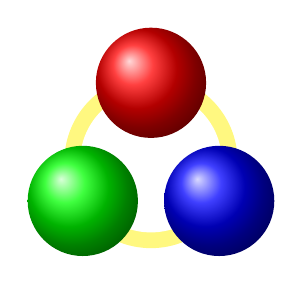
\begin{tikzpicture}
    \path[fill=yellow!50!white] (0,0) circle (11mm);
    \path[fill=white] (0,0) circle (9mm);
    \foreach \w/\c in {90/red,210/green,330/blue}
      {\path[shading=ball,ball color=\c] (\w:1cm) circle (7mm);}
  \end{tikzpicture}
\end{tcbexternal}
\end{dispExample}

\medskip

If a \refEnv{tcolorbox} is externalized, one should use
\refKey{/tcb/nobeforeafter} for the box. Indention and distances to
the text before and after have to be given separately outside the
\refEnv{tcbexternal} environment.

\begin{dispExample}
\noindent%
\begin{tcbexternal}[minipage]{example_tcolorbox}
  \begin{tcolorbox}[nobeforeafter,enhanced,
      fonttitle=\bfseries,title=Externalized Box,
      colframe=red!50!black,drop fuzzy shadow,
      interior style={fill overzoom image=goldshade.png}]
    This complete tcolorbox is externalized. One cannot use numbered
    boxes here. Note the \texttt{minipage} option which tells the
    current line width to the external snippet.
  \end{tcolorbox}
\end{tcbexternal}
\end{dispExample}

\begin{dispExample}
\begin{tcolorbox}[nobeforeafter,enhanced,
      fonttitle=\bfseries,title=Externalized Box,
      colframe=blue!50!black,
      interior style={fill overzoom image=blueshade.png}]
  \begin{tcbexternal}[minipage]{example_tcolorbox2}
    \color{white}%
    The interior of the tcolorbox is externalized.
    One can use numbered boxes without problems.
    Note that the text color has to be set for the text manually
    since it is converted into an image.
  \end{tcbexternal}
\end{tcolorbox}
\end{dispExample}

\begin{dispExample}
\begin{tcbexternal}[minipage]{example_tabularx}
  \newcolumntype{Y}{>{\raggedleft\arraybackslash}X}%
  \begin{tabularx}{\linewidth}{|l||Y|Y|Y|Y||Y|}\hline
    Group & One & Two & Three & Four & Sum\\\hline\hline
    Red & 1000.00 & 2000.00 & 3000.00 & 4000.00 & 10000.00\\\hline
    Green & 2000.00 & 3000.00 & 4000.00 & 5000.00 & 14000.00\\\hline
    Blue & 3000.00 & 4000.00 & 5000.00 & 6000.00 & 18000.00\\\hline\hline
    Sum & 6000.00 & 9000.00 & 12000.00 & 15000.00 & 42000.00\\\hline
  \end{tabularx}
\end{tcbexternal}
\end{dispExample}


\end{docEnvironment}

\begin{extTcbKey}[][doc new=2015-03-11]{name}{=\meta{name}}{no default,
  initially \texttt{unnamed}}
The \meta{name} is automatically prefixed with \refKey{/tcb/external/prefix}.
In combination, this has to be a unique file name for externalization.
Typically, this key is not used directly but is set indirectly as
mandatory parameter, see \refEnv{tcbexternal}.
\end{extTcbKey}


\clearpage
\begin{docEnvironment}[doc new=2015-03-11]{extcolorbox}{\oarg{options}\marg{name}\oarg{tcolorbox options}}
  This is an externalized version of \refEnv{tcolorbox} created
  using\\ \refCom{newtcbexternalizetcolorbox}:
\begin{dispListing}
\newtcbexternalizetcolorbox{extcolorbox}{tcolorbox}{}{}
\end{dispListing}
  \meta{options} and \meta{name} are given to the underlying \refEnv{tcbexternal}
  environment, while \meta{tcolorbox options} are given to \refEnv{tcolorbox}.

  \begin{marker}
  Note that you should not redefine \refKey{/tcb/before} and \refKey{/tcb/after}
  inside the \meta{tcolorbox options}, since the
  externalized version would not be identical to the non-externalized
  otherwise.
  \end{marker}

\begin{dispExample}
\begin{extcolorbox}[minipage]{example_extcolorbox}
  [ enhanced,colframe=red!50!black,colback=yellow!10,
    fonttitle=\bfseries,drop fuzzy shadow,
    title=My external box ]

  This box is completely externalized.

  \begin{tcolorbox}[colframe=blue,colback=blue!5,before skip=6pt]
  Inner box.
  \end{tcolorbox}
\end{extcolorbox}
\end{dispExample}
\end{docEnvironment}

\begin{marker}
\begin{itemize}
\item\textbf{Never} externalize numbered boxes.
\item\textbf{Never} externalize boxes which contain references to other
  things, e.g. using |\ref| or |\cite|.
\item\textbf{Never} externalize breakable boxes.
\end{itemize}
\kern6pt
\end{marker}

\clearpage
\begin{docEnvironment}[doc new=2015-03-11]{extikzpicture}{\oarg{options}\marg{name}\oarg{tikz options}}
  This is an externalized version of |tikzpicture| created
  using\\ \refCom{newtcbexternalizeenvironment}:
\begin{dispListing}
\newtcbexternalizeenvironment{extikzpicture}{tikzpicture}{}{}{}
\end{dispListing}
  \meta{options} and \meta{name} are given to the underlying \refEnv{tcbexternal}
  environment, while \meta{tikz options} are given to |tikzpicture|.

\tcbset{/tcb/external/externalize}%----- Do externalization even if switched off globally
\begin{dispExample}
\begin{center}
\begin{extikzpicture}[
  preamble={\usepackage{pgfplots}},  % add package for external graph
  input source on error=false,       % do not load source on error
]{example_pgfplots}
  \pgfplotsset{width=12cm}
  \begin{axis}[3d box=background,grid=major,
    xlabel=$x$, ylabel=$y$, zlabel=$z$, view/h=40,
    mesh/interior colormap name=hot,
    colormap/blackwhite,
    z buffer=sort,domain=0:90,y domain=0:60,
    zmin=0,zmax=2,z post scale=1.2,
    ]
  \addplot3[surf,mesh/interior colormap name=blackwhite,
    colormap/hot,] ( {cos(x)},{sin(x)}, {2*sin(y)} );
  \addplot3[surf] ( {2*cos(x)*cos(y)},{2*sin(x)*cos(y)}, {2*sin(y)} );
  \end{axis}
\end{extikzpicture}
\end{center}
\end{dispExample}

\end{docEnvironment}




\clearpage
\begin{docTcbKey}[][doc new=2015-03-11]{externalize listing}{=\meta{name}}{style, no default}
  The text content of a \refEnv{tcblisting} is externalized with the
  given \meta{name}. Note that the listing part is not externalized.
\end{docTcbKey}


\begin{dispExample}
\begin{tcblisting}{externalize listing=example_listing,
  bicolor,colback=yellow!10,colframe=yellow!50!black,
  colbacklower=white,center lower}
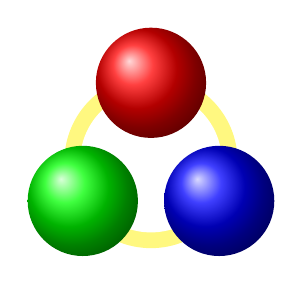
\begin{tikzpicture}
  \path[fill=yellow!50!white] (0,0) circle (11mm);
  \path[fill=white] (0,0) circle (9mm);
  \foreach \w/\c in {90/red,210/green,330/blue}
    {\path[shading=ball,ball color=\c] (\w:1cm) circle (7mm);}
\end{tikzpicture}
\end{tcblisting}
\end{dispExample}


\begin{docTcbKey}[][doc new=2015-03-11]{externalize listing\tcbexclamation}{=\meta{name}}{style, no default}
Combination of \refKey{/tcb/externalize listing} and \refKey{/tcb/external/force remake}.
\end{docTcbKey}

\begin{docTcbKey}[][doc new=2015-03-11]{externalize example}{=\meta{name}}{style, no default}
  The text content of a \refEnv{dispExample*} is externalized with the
  given \meta{name}. Note that the listing part is not externalized.

\begin{dispExample}
\begin{dispExample*}{sidebyside,externalize example=example_example}
\tikz\path[shading=ball,
  ball color=red] circle (7mm);
\end{dispExample*}
\end{dispExample}
\end{docTcbKey}

\begin{docTcbKey}[][doc new=2015-03-11]{externalize example\tcbexclamation}{=\meta{name}}{style, no default}
Combination of \refKey{/tcb/externalize example} and \refKey{/tcb/external/force remake}.
\end{docTcbKey}

\clearpage
\subsection{Customization}\label{subsec:external_custom}

\begin{extTcbKey}[][doc new=2015-03-11]{safety}{=\meta{length}}{no default,
  initially |2mm|}
The snippet box is surrounded with a safety border with a thickness of
\meta{length}. This border is automatically trimmed during picture inclusion.
The reason for this mechanism is to catch  box content which
extrudes over the bounding box. For example, shadows of a |tcolorbox| are
painted outside the bounding box and would be lost otherwise.
\end{extTcbKey}

\begin{extTcbKey}[][doc new=2015-03-11]{environment}{=\meta{env}}{no default, initially unset}
Surrounds the exported snippet text with an environment \meta{env} without
parameters.
Note that this option is ignored for \refKey{/tcb/externalize listing}.
\end{extTcbKey}

\begin{extTcbKey}[][doc new=2015-05-05]{environment with percent}{\colOpt{=true\textbar false}}{default |true|,
  initially |true|}
If set to |true|, the |\begin| and |\end| code of \refKey{/tcb/external/environment}
is appended with a percent sign. For verbatim environments, this option
typically has to be se to |false|.
\end{extTcbKey}


\begin{extTcbKey}[][doc new=2015-03-11]{minipage}{\colOpt{=\meta{length}}}{default \texttt{\cs{linewidth}},
  initially unset}
Surrounds the exported snippet text with a minipage. The optional \meta{length}
parameter sets the width of the minipage. Note that the default width is the
current line width of the main document.
See \refEnv{tcbexternal} for examples.
Note that this option is ignored for \refKey{/tcb/externalize listing}.
\end{extTcbKey}


\begin{extTcbKey}[][doc new=2015-03-11]{plain}{}{no value, initially set}
  Removes any text which was set to surround the snippet.
  This removes the setting of  \refKey{/tcb/external/minipage}, but is
  independent of \refKey{/tcb/external/safety}.
\end{extTcbKey}


\begin{extTcbKey}[][doc new=2015-03-11]{compiler}{=\meta{text}}{no default,
  initially \texttt{pdflatex}}
  Sets the name of the compiler for the snippets. Note that this compiler
  has to support the |\pdfmdfivesum| primitive e.g. using the
  |pdftexcmds| package. This should work for |xelatex| and |lualatex|.
\end{extTcbKey}

\begin{extTcbKey}[][doc new=2015-03-11]{runs}{=\meta{number}}{no default,
  initially |1|}
  Sets the number of compiler runs for the snippet.
\begin{dispExample}
\begin{tcbexternal}[minipage,runs=2]{example_raster}
  \begin{tcbitemize}[raster equal height,
      size=small,colframe=red!50!black,colback=red!10!white]
    \tcbitem One
    \tcbitem \Huge Two
    \tcbitem Three
    \tcbitem Four
  \end{tcbitemize}
\end{tcbexternal}
\end{dispExample}
\end{extTcbKey}

\enlargethispage*{1cm}
\begin{extTcbKey}[][doc new=2015-03-11]{input source on error}{\colOpt{=true\textbar false}}{default |true|,
  initially |true|}
If set to |true|, the source code of the snippet is loaded instead of
the failed pdf picture. Typically, this will lead to an error stop at the
faulty place of the source and such helps detecting the cause.
If the source input compiles without error, the document setup
may be incorrect, see \Fullref{subsec:external_preparation}.
Maybe, the |external/| subdirectory has to be created manually in this case,
see \refKey{/tcb/external/prefix}.\par
If the option is set to |false|, the compilation stops immediately on an error.
The log file of the external snippet has to be consulted for error messages
in this case.
\end{extTcbKey}


\clearpage

\begin{extTcbKey}[][doc new=2015-05-05]{preclass}{=\meta{code}}{no default,
  initially unset}
  The given \meta{code} is added before the snippet document.
  Typically, this means before |\documentclass|.
  This is not used for compilation of the main document.
\end{extTcbKey}


\begin{extTcbKey}[][doc new=2015-05-05]{PassOptionsToPackage}{=\marg{options}\marg{package}}{no default,
  initially unset}
  The given \meta{options} are passed to the given \meta{package} for
  the snippet document. This is a shortcut for using \refKey{/tcb/external/preclass}
  with |\PassOptionsToPackage|.
  This not used for compilation of the main document.
\end{extTcbKey}


\begin{extTcbKey}[][doc new=2015-05-05]{PassOptionsToClass}{=\marg{options}\marg{class}}{no default,
  initially unset}
  The given \meta{options} are passed to the given \meta{class} for
  the snippet document. This is a shortcut for using \refKey{/tcb/external/preclass}
  with |\PassOptionsToClass|.
  This not used for compilation of the main document.
\end{extTcbKey}


\begin{extTcbKey}[][doc new=2015-05-05]{clear preclass}{}{no value}
  Removes all additional \refKey{/tcb/external/preclass} settings.
\end{extTcbKey}



\begin{extTcbKey}[][doc new=2015-03-11]{preamble}{=\meta{code}}{no default,
  initially unset}
  The given \meta{code} is added to the preamble of the snippet document.
  This is not used for compilation of the main document.
\end{extTcbKey}


\begin{extTcbKey}[][doc new=2015-05-05]{preamble tcbset}{=\meta{options}}{no default,
  initially unset}
  The given \meta{options} are added as parameter for \refCom{tcbset}
  to the preamble of the snippet document.
  This are not used for compilation of the main document.
\end{extTcbKey}


\begin{extTcbKey}[][doc new=2015-03-16]{clear preamble}{}{no value}
  Removes all additional \refKey{/tcb/external/preamble} settings.
\end{extTcbKey}



\begin{docCommand}[doc new=2015-03-11]{tcbifexternal}{\marg{true}\marg{false}}
  Expands to \meta{true}, if executed during snippet compilation,
  and to \meta{false}, if executed during main document compilation.
  This can be used \emph{before} \refCom{tcbEXTERNALIZE} to
  give different setting to snippet and main document.
\begin{dispListing}
\tcbifexternal{
  \usepackage{onlyforexternal}
}{
  \usepackage{onlyformain}
}
\end{dispListing}
\end{docCommand}



\clearpage
\begin{docCommand}[doc new=2015-03-11]{newtcbexternalizeenvironment}{\marg{newenv}\marg{env}\marg{options}\marg{begin}\marg{end}}
  Creates a new environment \meta{newenv} which is based on
  \refEnv{tcbexternal}. This enviroment takes \emph{at least}
  one optional parameter and one mandatory parameter.
  These two parameters are passed to \refEnv{tcbexternal}.
  Further, the given \meta{options} are always added to the option list of \refEnv{tcbexternal}.\par
  The environment content is externalized and the external snippet is surrounded
  by an environment \meta{env}. All further parameters of \meta{newenv}
  are given to \meta{env} as parameters.\par
  The included image is prepended by \meta{begin} and appended by \meta{end}.\par
  \refEnv{extikzpicture} is an example application
  for \refCom{newtcbexternalizeenvironment}.

\begin{dispExample}
\newtcbexternalizeenvironment{extabular}{tabular}{}{\par\centering}{\par}

\begin{extabular}{example_tabular}{|l|p{6cm}|r|}\hline
A & B & C\\\hline
a & This table is externalized as snippet. Obviously,
  this only makes sense for highly complex tables.
& b\\\hline
\end{extabular}
\end{dispExample}
\end{docCommand}


\begin{docCommand}[doc new=2015-03-11]{renewtcbexternalizeenvironment}{\marg{newenv}\marg{env}\marg{options}\marg{begin}\marg{end}}
  Identical to \refCom{newtcbexternalizeenvironment}, but the environment \meta{newenv}
  is created by |\renewenvironment| instead of |\newenvironment|.
\end{docCommand}


\begin{docCommand}[doc new=2015-03-11]{newtcbexternalizetcolorbox}{\marg{newenv}\marg{env}\marg{options}\marg{begin end options}}
  Creates a new environment \meta{newenv} which is based on
  \refEnv{tcbexternal}. This enviroment takes \emph{at least}
  one optional parameter and one mandatory parameter.
  These two parameters are passed to \refEnv{tcbexternal}.
  Further, the given \meta{options} are always added to the option list of \refEnv{tcbexternal}.\par
  The environment content is externalized and the external snippet is surrounded
  by an environment \meta{env}. All further parameters of \meta{newenv}
  are given to \meta{env} as parameters.
  \textbf{In contrast to \refCom{newtcbexternalizeenvironment}, the
  environment \meta{env} is intended to be based on \refEnv{tcolorbox}
  or \refEnv{tcblisting}.}\par
  The \meta{begin end options} are options for settings the space before
  and after the included image using \refKey{/tcb/before}, \refKey{/tcb/before skip},
  \refKey{/tcb/after}, or \refKey{/tcb/after skip}.
  \begin{marker}
  Use the exact identical values for \refKey{/tcb/before} and \refKey{/tcb/after}
  inside \meta{begin end options} as they where used for definition of
  \meta{env}! Otherwise, externalized and non-externalized version will have
  different spacings.
  \end{marker}
  \refEnv{extcolorbox} is an example application for \refCom{newtcbexternalizetcolorbox}.


\inputpreamblelisting{M}

{
\tcbset{external/preamble={\input{tcolorbox_preamble_M.tex}}}
\begin{dispExample}
\begin{exmyownlisting}{example_mylisting}% <- name for the external file
  {My externalized example box}
This is my \LaTeX\ box.
\end{exmyownlisting}
\end{dispExample}
}
\end{docCommand}


\begin{docCommand}[doc new=2015-03-11]{renewtcbexternalizetcolorbox}{\marg{newenv}\marg{env}\marg{options}\marg{begin end options}}
  Identical to \refCom{newtcbexternalizetcolorbox}, but the environment \meta{newenv}
  is created by |\renewenvironment| instead of |\newenvironment|.
\end{docCommand}


\begin{docCommand}[doc new=2016-07-14]{tcbiffileprocess}{\marg{condition}\marg{source}\marg{md5-file}\marg{target}\marg{true}\marg{false}}
  This is a low-level macro which is internally used.
  The MD5 digest of a \meta{source} file is compared with
  a stored MD5 digest from an auxiliary \meta{md5-file}.
  If they are not equal, the auxiliary \meta{md5-file} is updated to
  store the current MD5 digest. Further,
  \begin{itemize}
  \item if \meta{condition} equals |0|, \meta{true} is executed.
  \item if \meta{condition} equals |1|:\\
    If the current and stored MD5 digests were different, \meta{true} is executed.\\
    Otherwise, if the \meta{target} file is not existing, \meta{true} is executed.\\
    Otherwise, if the \meta{target} file is older than the \meta{md5-file}, \meta{true} is executed.\\
    Otherwise, \meta{false} is executed.
  \item if \meta{condition} equals |2|, \meta{false} is executed.
  \end{itemize}
  The intended processing purpose of the \meta{true} code is to produce a \meta{target}
  file from the given \meta{source} file.
\end{docCommand}


\clearpage
\subsection{Troubleshooting and FAQ}\label{subsec:external_troubleshooting}

\begin{itemize}

\item\textbf{I use the default settings, but the |external| subdirectory is
  not created.}\\
  Depending on operating system and compiler, an |external| subdirectory is
  automatically created or not. If not, create such a directory manually
  or add the following to your document\footnote{The |shellesc| package
  is loaded automatically by the library.}:
\begin{dispListing}
\ShellEscape{mkdir external}
\end{dispListing}
or
\begin{dispListing}
\ShellEscape{mkdir -p external}
\end{dispListing}
  If the combination of \refKey{/tcb/external/prefix} and chosen snippet
  name points to another subdirectory than |external|, this has to be
  adapted.

\item\textbf{I use the |minted| package and I get a cache directory for
  every externalized snippet.}\\
  To avoid this problem, there are several ways.
  \begin{itemize}
  \item If you do not need |minted| inside the snippet code, you may use
    |\usepackage{minted}| \emph{after} \refCom{tcbEXTERNALIZE}
    or use \refCom{tcbifexternal} to switch |minted| off for the external code.
    If |minted| is already included by another package, add the following to
    your preamble:
\begin{dispListing}
\tcbset{external/PassOptionsToPackage={draft}{minted}}
\end{dispListing}
  \item If |minted| is needed for the snippet code, caching can be switched
    off by adding the following to your preamble:
\begin{dispListing}
\tcbset{external/PassOptionsToPackage={cache=false}{minted}}
\end{dispListing}
  Alternatively, the |cachedir| option of |minted| may be used to redirect
  the cache.
  \end{itemize}


\end{itemize}

